\section{Scientific Background}%
\label{sec:introduction}

\begin{frame}
    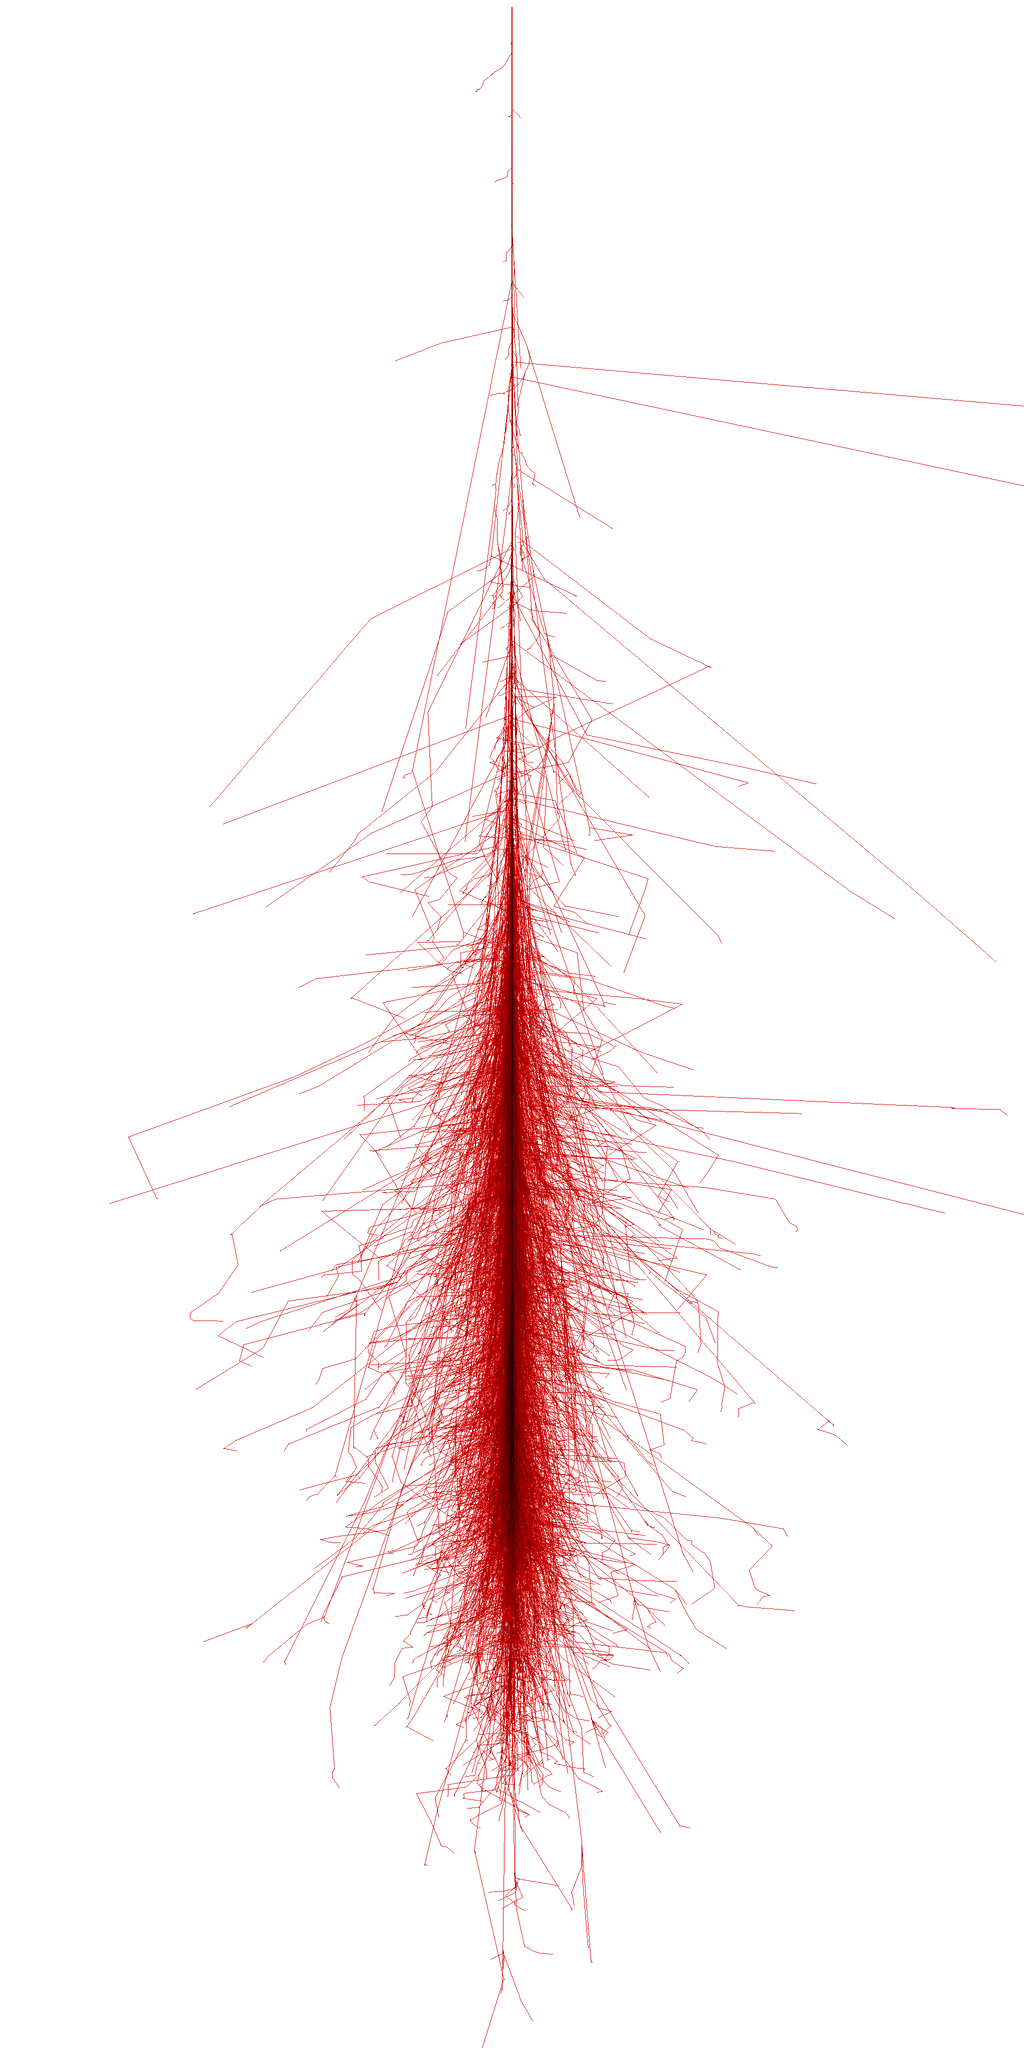
\includegraphics[height=0.5\textwidth]{graphics/photon100.png}
\end{frame}

\begin{frame}{Extensive Air Showers}
    \ifthenelse{\equal{\theme}{\string 1}}
    {% use dark theme
    
\includegraphics[width=0.48\textwidth]{build/tikz//heitler_model_dark.pdf}
    \includegraphics[width=0.48\textwidth]{build/tikz/cherenkov_radiation_dark.pdf}
    }
    {% use light theme
    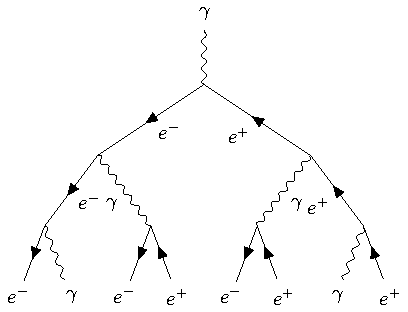
\includegraphics[width=0.48\textwidth]{build/tikz/heitler_model.pdf}
    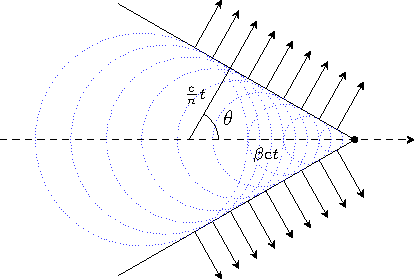
\includegraphics[width=0.48\textwidth]{build/tikz/cherenkov_radiation.pdf}
    }
\end{frame}

\begin{frame}{The Cherenkov Telescope Array (CTA)}
    \begin{minipage}{0.55\textwidth}
      \begin{itemize}
        \setlength\itemsep{1em}
        \item 2 sites: CTA North and CTA South
        \item 3 types of telescopes:
        \begin{itemize}
          \setlength\itemsep{0.5em}
          \item [•] Small-Sized Telescope (SST): \;\(\SI{5}{\tera\eV}\) -- \(\SI{300}{\tera\eV}\)
          \item [•] Medium-Sized Telescope (MST): \;\(\SI{150}{\giga\eV}\) -- \(\SI{5}{\tera\eV}\)
          \item [•] Large-Sized Telescope (LST): \;\(\SI{20}{\giga\eV}\) -- \(\SI{150}{\giga\eV}\)
        \end{itemize}
      \end{itemize}
    \end{minipage}
    \begin{minipage}{0.42\textwidth}
      \begin{center}
        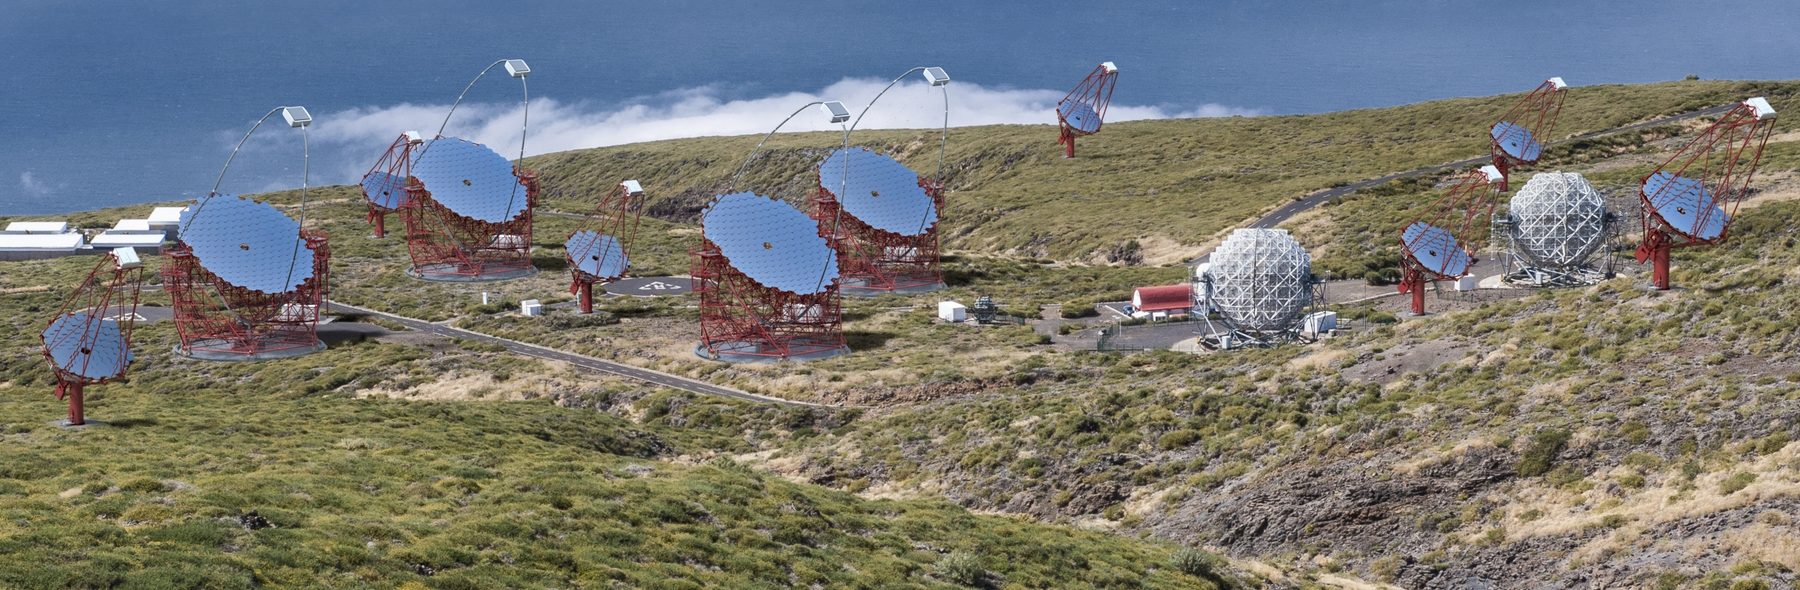
\includegraphics[width=\textwidth]{graphics/cta_north_render.jpg}
        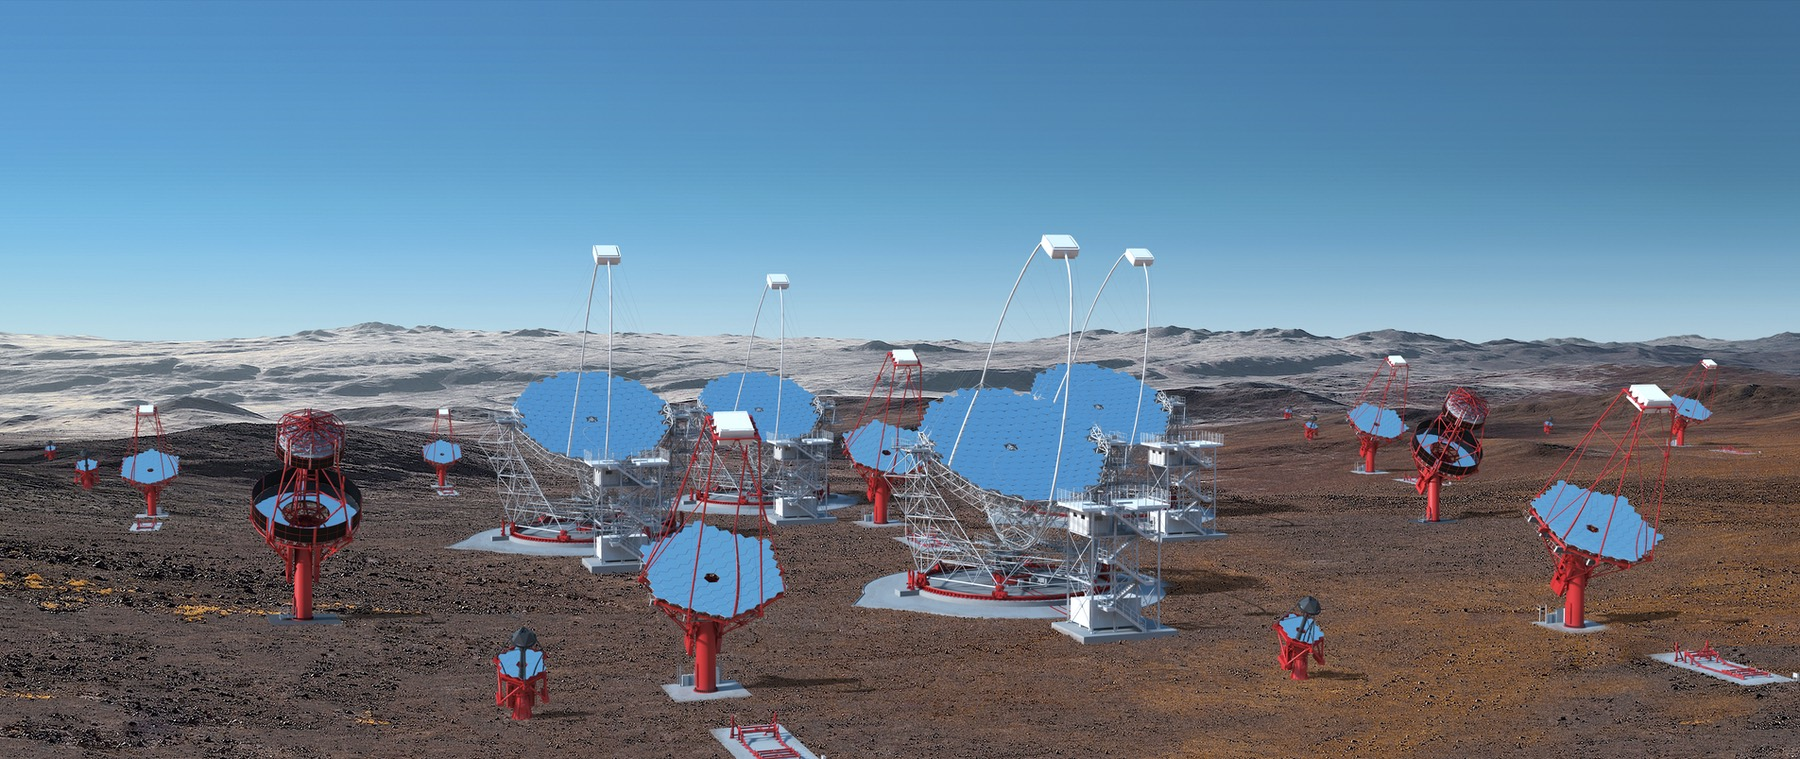
\includegraphics[width=\textwidth]{graphics/cta_south_render.jpg}
        \vspace{-0.25cm}
        \ifthenelse{\equal{\theme}{\string 1}}
        {% use dark theme
        \blfootnote{\href{https://www.cta-observatory.org/about/how-cta-works/}{\textcolor{white!85!black}{Image Credit: G.~Pérez Diaz (IAC) and M.-A.~Besel (CTAO)}}}
        }
        {% use light theme
        \blfootnote{\href{https://www.cta-observatory.org/about/how-cta-works/}{\textcolor{darkgray!85!black}{Image Credit: G.~Pérez Diaz (IAC) and M.-A.~Besel (CTAO)}}}
        }
      \end{center}
    \end{minipage}
  \end{frame}
